\documentclass[11pt,a4paper]{article}

\usepackage[utf8]{inputenc}
\usepackage[T1]{fontenc}
\usepackage{lmodern}
\usepackage[margin=2.5cm]{geometry}
\usepackage{hyperref}
\usepackage{enumitem}
\usepackage{xcolor}
\usepackage{listings}
\usepackage{booktabs}
\usepackage{tcolorbox}
\usepackage{parskip}
\usepackage{tikz}
\usetikzlibrary{positioning,arrows.meta,shapes.geometric,fit,backgrounds}

\hypersetup{
  colorlinks=true,
  linkcolor=blue!60!black,
  urlcolor=blue!60!black,
  citecolor=blue!60!black
}

\lstset{
  basicstyle=\ttfamily\small,
  backgroundcolor=\color{gray!8},
  frame=single,
  framerule=0pt,
  breaklines=true,
  showstringspaces=false,
  columns=fullflexible,
  xleftmargin=6pt,
  xrightmargin=6pt,
  aboveskip=6pt,
  belowskip=6pt
}

\newtcolorbox{notebox}{
  colback=yellow!8,
  colframe=yellow!50!black,
  boxrule=0.4pt,
  arc=2pt,
  left=6pt,right=6pt,top=4pt,bottom=4pt
}

\title{From Pipeline to Chatbot:\\
       Next Steps for the SciFact Claim Verification System}
\author{Group 27 -- UZH CL RAG Course, FS 2026}
\date{\today}

\begin{document}
\maketitle

\section{Motivation}

The current \texttt{scifact-claim-verification} system is a research pipeline
that processes the SciFact dev set in batch through a sequence of offline
scripts (\texttt{scripts/01\_\ldots{}} through \texttt{12\_\ldots{}}). It
produces strong numbers on a fixed benchmark but is not yet usable
interactively: a user cannot type a claim and see a verdict with cited
evidence.

The next phase is to expose the pipeline as a \textbf{chatbot} with a
frontend and a backend, so that:

\begin{itemize}
  \item arbitrary claims can be entered in natural language,
  \item results (verdict, confidence, evidence, explanation) are shown in a
        conversational interface,
  \item the system runs on the three networked Nuvolos apps
        (\textit{Frontend}, \textit{Backend}, \textit{Database}) rather
        than as local scripts.
\end{itemize}

This document outlines the concrete steps to get there.

\section{Current State}

\textbf{What exists:}
\begin{itemize}
  \item \texttt{retrieval/pipeline.py} -- hybrid retrieval (BM25 + dense
        with RRF fusion, optional cross-encoder reranking).
  \item \texttt{reasoning/joint.py} -- fine-tuned DeBERTa-v3-large joint
        sentence-level classifier (SUPPORT / CONTRADICT / NEI).
  \item \texttt{calibration/} -- NLI-confidence and retriever-disagreement
        abstention gate.
  \item \texttt{generation/llm\_generator.py} -- Gemma 4 E4B cited
        explanation generator (plus extractive and template fallbacks).
  \item Evaluation scripts with strong results on SciFact dev
        (abstract-level F1 = 0.401, accuracy with abstention = 0.81).
\end{itemize}

\textbf{What is missing:}
\begin{itemize}
  \item No single-query entry point -- everything runs on the full dev set.
  \item No HTTP layer.
  \item No user-facing UI.
  \item The dense index is rebuilt from local FAISS files on each run, so
        there is no persistent store the Backend app could query.
  \item No chat-specific logic (claim extraction from free text,
        follow-up rewriting).
\end{itemize}

\section{Target Architecture}

The three networked Nuvolos apps map naturally onto a standard
RAG-chatbot deployment:

\begin{center}
\begin{tabular}{@{}lll@{}}
\toprule
\textbf{Nuvolos app} & \textbf{Role} & \textbf{Stack} \\
\midrule
Frontend (2 NCU) & Chat UI          & Streamlit + \texttt{st.chat\_*} \\
Backend  (2 NCU) & HTTP API, pipeline & FastAPI + \texttt{uvicorn} \\
Database (2 NCU) & Corpus + embeddings & PostgreSQL + \texttt{pgvector} \\
Trainer (GPU)   & Gemma 4 inference (opt.) & PyTorch \\
\bottomrule
\end{tabular}
\end{center}

Large model weights and the SciFact corpus live on the shared mount
\texttt{/space\_mounts/pars} so that the Frontend and Backend do not each
re-download them.

\subsection{Infrastructure Diagram}

Figure~\ref{fig:infra} shows the deployment topology on the Nuvolos
Master instance. Instance-wide networking (\texttt{ipc\_mode: instance})
lets the Frontend, Backend, and Database reach each other over fixed
hostnames without public routing. The Editor runs in an isolated
namespace and is used only for file management.

\begin{figure}[h]
\centering
\resizebox{\textwidth}{!}{%
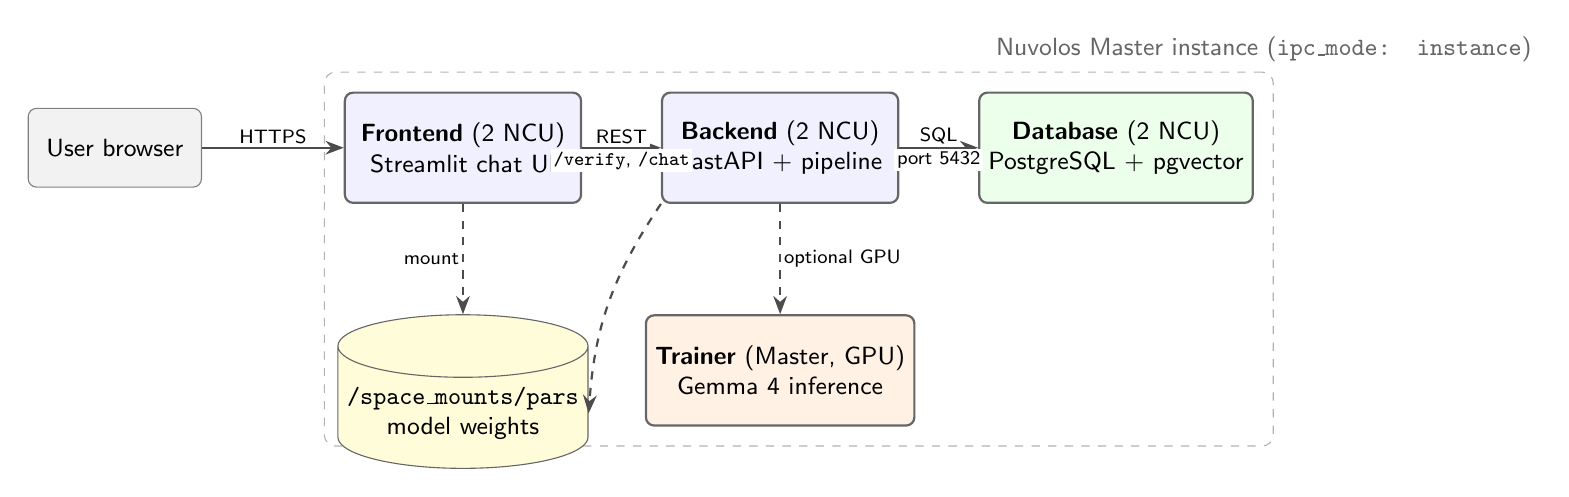
\begin{tikzpicture}[
  font=\small\sffamily,
  node distance=8mm and 10mm,
  app/.style={
    rectangle, rounded corners=3pt, draw=black!60, thick,
    minimum width=30mm, minimum height=14mm, align=center,
    fill=blue!6
  },
  db/.style={app, fill=green!8},
  gpu/.style={app, fill=orange!10},
  user/.style={
    rectangle, rounded corners=3pt, draw=black!50,
    minimum width=22mm, minimum height=10mm, align=center, fill=gray!10
  },
  store/.style={
    cylinder, shape border rotate=90, aspect=0.25,
    draw=black!60, fill=yellow!15,
    minimum width=26mm, minimum height=12mm, align=center
  },
  arr/.style={-Stealth, thick, draw=black!70},
  lbl/.style={font=\scriptsize\sffamily, fill=white, inner sep=1pt}
]

\node[user] (user) {User browser};

\node[app, right=18mm of user] (front) {\textbf{Frontend} (2 NCU)\\Streamlit chat UI};
\node[app, right=of front] (back) {\textbf{Backend} (2 NCU)\\FastAPI + pipeline};
\node[db, right=of back] (dbapp) {\textbf{Database} (2 NCU)\\PostgreSQL + pgvector};

\node[gpu, below=14mm of back] (trainer) {\textbf{Trainer} (Master, GPU)\\Gemma 4 inference};
\node[store, below=14mm of front] (mount) {\texttt{/space\_mounts/pars}\\model weights};

\draw[arr] (user) -- node[lbl,above]{HTTPS} (front);
\draw[arr] (front) -- node[lbl,above]{REST} node[lbl,below]{\texttt{/verify}, \texttt{/chat}} (back);
\draw[arr] (back) -- node[lbl,above]{SQL} node[lbl,below]{port 5432} (dbapp);
\draw[arr, dashed] (back) -- node[lbl,right]{optional GPU} (trainer);
\draw[arr, dashed] (front) -- node[lbl,left]{mount} (mount);
\draw[arr, dashed] (back.south west) to[bend right=15] (mount.east);

\begin{pgfonlayer}{background}
  \node[draw=black!30, dashed, rounded corners,
        fit=(front)(back)(dbapp)(trainer),
        inner sep=7pt, label={[black!60]above right:Nuvolos Master instance (\texttt{ipc\_mode: instance})}] {};
\end{pgfonlayer}

\end{tikzpicture}%
}
\caption{Deployment topology. Solid arrows are request paths; dashed
arrows are optional dependencies (shared model mount, GPU offload).
All three networked apps live in the same Nuvolos instance and resolve
each other by fixed internal hostnames.}
\label{fig:infra}
\end{figure}

\section{Next Steps}

\subsection{Step 1 -- Service Layer}

Introduce a single class that wraps the whole pipeline and exposes a
one-shot \texttt{verify(claim)} method. This is the foundation for both
the API and any future batch use.

\begin{lstlisting}[language=Python]
# src/claimverify/service.py
class ClaimVerifier:
    def __init__(self, config): ...
    def verify(self, claim: str) -> VerifyResult: ...
\end{lstlisting}

\texttt{VerifyResult} returns:
\begin{itemize}
  \item \texttt{verdict} -- SUPPORT / CONTRADICT / NEI,
  \item \texttt{confidence} -- softmax score of the chosen label,
  \item \texttt{abstained} -- bool from the abstention gate,
  \item \texttt{evidence} -- list of
        \texttt{\{doc\_id, title, sentence, score\}},
  \item \texttt{explanation} -- string with \texttt{[N]} citation markers,
  \item \texttt{retriever\_disagreement} -- Jaccard@10 between BM25 and
        dense.
\end{itemize}

Models are loaded lazily and kept in memory; cold-start for
DeBERTa-v3-large + Gemma 4 is several seconds and must not happen per
request.

\subsection{Step 2 -- Persistent Index in pgvector}

Move the dense index from in-process FAISS files into the Database app
so the Backend can query it over the local network without local GPU or
disk pressure.

\textbf{Schema:}
\begin{lstlisting}[language=SQL]
CREATE TABLE documents (
    doc_id     TEXT PRIMARY KEY,
    title      TEXT,
    abstract   TEXT,
    sentences  JSONB
);

CREATE TABLE embeddings (
    doc_id        TEXT REFERENCES documents(doc_id),
    sentence_idx  INT,
    embedding     VECTOR(1024),  -- bge-m3
    PRIMARY KEY (doc_id, sentence_idx)
);

CREATE INDEX ON embeddings
    USING hnsw (embedding vector_cosine_ops);
\end{lstlisting}

A one-shot script \texttt{scripts/ingest\_to\_pgvector.py} loads the
SciFact corpus, embeds each sentence with \texttt{BAAI/bge-m3}, and
inserts into the Database app.

BM25 stays in-process (\texttt{rank\_bm25}) initially -- moving it to
Postgres full-text search is possible but adds complexity for little
gain at SciFact scale ($\sim$5\,k abstracts).

\subsection{Step 3 -- Backend API (FastAPI)}

\begin{center}
\begin{tabular}{@{}lll@{}}
\toprule
\textbf{Endpoint} & \textbf{Purpose} & \textbf{Request body} \\
\midrule
\texttt{POST /verify} & Single-claim verification & \texttt{\{claim\}} \\
\texttt{POST /chat}   & Conversational wrapper    & \texttt{\{messages[]\}} \\
\texttt{GET  /health} & Liveness probe            & --- \\
\texttt{GET  /models} & Loaded model names        & --- \\
\bottomrule
\end{tabular}
\end{center}

\texttt{/chat} is what makes the system a chatbot rather than a form: it
accepts a message history, extracts/rewrites the latest user turn into a
verifiable claim (see Step~5), calls \texttt{verify}, and formats the
reply.

Sessions are stateless at first; if time allows, add a \texttt{session\_id}
with in-memory history so follow-up questions (``\textit{what about in
children?}'') can be resolved against earlier turns.

\subsection{Step 4 -- Frontend (Streamlit)}

A minimal chat UI built with \texttt{st.chat\_input} and
\texttt{st.chat\_message}. Each assistant response should show:

\begin{itemize}
  \item a colour-coded verdict badge (green / red / grey),
  \item a confidence bar,
  \item an abstention notice when the gate triggers,
  \item an expandable ``Evidence'' panel listing cited sentences with
        their source abstract titles,
  \item a small disagreement indicator (Jaccard\,@\,10) to make the core
        research signal visible to the user.
\end{itemize}

The Frontend talks to the Backend via its internal Nuvolos hostname
(visible in the \textit{Applications $\to$ Configure} panel). No public
routing is required.

\subsection{Step 5 -- Chat-Specific Logic}

The current pipeline assumes its input is already a well-formed claim.
In a chat setting this is rarely true, so two small additions are
needed:

\begin{enumerate}
  \item \textbf{Claim extraction.} A short Gemma prompt that converts
        free-form user input (\textit{``tell me about aspirin and
        cancer''}) into a verifiable claim
        (\textit{``Aspirin reduces the risk of colorectal cancer.''}),
        or returns ``no claim detected''.
  \item \textbf{Follow-up rewriting.} Using the conversation history,
        rewrite pronouns and ellipses into a standalone claim before
        retrieval (\textit{``what about in adults?''} $\to$
        \textit{``Aspirin reduces the risk of colorectal cancer in
        adults.''}).
\end{enumerate}

When abstention fires, this should be surfaced explicitly in the chat
reply (\textit{``The evidence is inconclusive\ldots''}) rather than
silently returning NEI.

\subsection{Step 6 -- Custom Queries and (Optionally) Custom Corpus}

Accepting custom \emph{queries} comes for free once Steps~1--4 are done:
the chat box accepts arbitrary text.

Accepting custom \emph{documents} (beyond SciFact) is a stretch goal.
It would require:
\begin{itemize}
  \item \texttt{POST /corpus/add} to embed and insert a new abstract,
  \item a chunking / deduplication policy,
  \item a trust model (users can poison the corpus with bad evidence).
\end{itemize}
Defer this unless the course scope clearly asks for it.

\subsection{Step 7 -- Deployment on Nuvolos}

\begin{itemize}
  \item Place all model weights under \texttt{/space\_mounts/pars/models/}
        so both the Frontend and Backend apps see them.
  \item Backend: \texttt{uvicorn claimverify.api:app --host 0.0.0.0
        --port 8000}.
  \item Frontend: read \texttt{BACKEND\_URL} from an env var so the
        hostname is not hard-coded.
  \item GPU for Gemma 4 requires scaling the \textit{Trainer} app from
        the Nuvolos web UI (cannot be done from the CLI). For a
        CPU-only demo, fall back to
        \texttt{generation.method\,=\,extractive}.
\end{itemize}

\begin{notebox}
\textbf{Credit budget.} Running Frontend + Backend + Database
simultaneously burns $\sim$6 NCU-hours per hour. Stop all three apps
when not demoing.
\end{notebox}

\section{Build Order}

\begin{enumerate}
  \item \texttt{service.py} + \texttt{scripts/demo\_verify.py}
        (proves end-to-end still works on a single string).
  \item FastAPI wrapper around the service.
  \item Streamlit chat UI hitting \texttt{/verify}.
  \item Swap FAISS $\to$ pgvector.
  \item Claim extraction and follow-up rewriting.
  \item \textit{(Optional)} Custom-corpus upload.
\end{enumerate}

Steps 1--3 produce a demo-able chatbot on the existing FAISS index;
Step 4 is the refactor that makes it production-shaped on Nuvolos;
Step 5 turns it from a ``claim-input form'' into an actual chat
experience.

\section{MultiVerS Integration}

Alongside the chatbot work, the MultiVerS ablations
(Wadden 2022) suggest a concrete upgrade path for the verdict module.
Their Table~3c ablation on modelling approach shows that predicting
labels from selected rationales alone collapses ($-66\%$ F1 on
context-dependent instances) compared to a multitask model that sees
the full abstract ($-14\%$). Our current sentence-level joint model is
structurally close to their worst variant on this axis, which plausibly
explains a large share of the $40.1 \to 72.5$ F1 gap.

MultiVerS is MIT-licensed and publishes the exact \texttt{scifact}
checkpoint behind their 72.5 number
(\url{https://github.com/dwadden/multivers}).

\subsection{Three Integration Levels}

\begin{description}
  \item[Level 1 -- Baseline run (hours).]
    Pull their \texttt{scifact} checkpoint via
    \texttt{script/get\_checkpoint.py}, run \texttt{predict.py} on
    SciFact dev in an isolated environment, compare head-to-head with
    our 40.1. No changes to our code. Converts the cross-paper comparison
    in our results table into a clean dev-set number.
  \item[Level 2 -- Drop-in verdict module (days).]
    Replace \texttt{reasoning/joint.py} with a wrapper that calls the
    MultiVerS model on full abstracts, keep our hybrid retrieval and
    disagreement-based abstention on top. Gives us the
    full-document-context architecture their ablations endorse, while
    preserving our research angle (retriever disagreement as an
    uncertainty signal).
  \item[Level 3 -- Reproduce pretraining (weeks).]
    Not worth it. They release \texttt{fever\_sci} and \texttt{scifact}
    checkpoints, which already bake in the weak-supervision step their
    Table~3a measures.
\end{description}

\subsection{Dependency Skew}

Level~2 is gated by a version gap between the two codebases:

\begin{center}
\begin{tabular}{@{}lll@{}}
\toprule
 & \textbf{MultiVerS (pinned)} & \textbf{This project} \\
\midrule
torch             & 1.7.1  & $\geq$ 2.1 \\
transformers      & 4.2.2  & $\geq$ 4.40 \\
pytorch-lightning & 1.2.1  & not used \\
Python            & 3.7-era & 3.10+ \\
\bottomrule
\end{tabular}
\end{center}

Three ways to handle the gap, in increasing order of effort:

\begin{enumerate}
  \item \textbf{Separate venv + subprocess.} Run their \texttt{predict.py}
        unmodified, hand claims in and predictions out via temp files.
        Fastest path; ugly but acceptable for a baseline number.
  \item \textbf{MultiVerS as its own Nuvolos service.}
        Deploy their code on the \textit{Trainer} app (which already
        has GPU for Gemma~4) as a small FastAPI wrapper. Our Backend
        calls it over the instance network. Clean isolation, fits the
        chatbot architecture in Fig.~\ref{fig:infra}. Estimated 1--2 days.
  \item \textbf{Port the model forward.} Reimplement the Longformer
        encoder with a label head and token-level rationale head
        against modern Hugging Face (\texttt{LongformerModel} + two
        heads, two-term loss). Load their released weights with a key
        rename. 3--5 days; cleanest long-term but not required for the
        course deadline.
\end{enumerate}

\subsection{Recommendation}

\begin{enumerate}
  \item \textbf{Do Level~1 this week.} It is a free datapoint for the
        course report and turns an apples-to-oranges comparison
        (\textit{our dev} vs \textit{their test}) into a clean dev-set
        head-to-head.
  \item \textbf{If the numbers justify it, do Level~2 via option~(b).}
        The MultiVerS service slots naturally onto the Trainer app next
        to Gemma~4, and the Backend's \texttt{/verify} endpoint becomes
        a thin orchestrator: retrieval $\to$ MultiVerS $\to$ abstention
        $\to$ generation.
\end{enumerate}

This plan also updates the chatbot build order: Level~1 can run in
parallel with Step~1 of the chatbot work, and Level~2 (option b) becomes
a fourth service alongside Frontend, Backend, and Database in
Fig.~\ref{fig:infra}.

\section{Open Questions}

\begin{itemize}
  \item \textbf{Streamlit vs.\ Gradio?} Streamlit has first-class chat
        primitives since 1.24; Gradio is lighter but less flexible for
        sidebars and evidence panels. Recommend Streamlit.
  \item \textbf{Keep FAISS?} For $\sim$5\,k abstracts, FAISS in-process
        is faster than network calls to pgvector. The argument for
        pgvector is architectural (matches the Nuvolos app layout and
        the course brief), not performance.
  \item \textbf{Chat memory.} How far back should follow-up rewriting
        look? A sliding window of the last 4 turns is probably enough
        and avoids unbounded prompt growth.
  \item \textbf{MultiVerS licensing vs pretraining data.} The code and
        \texttt{scifact} checkpoint are MIT, but FEVER-SCI weak
        supervision draws on PubMedQA and EvidenceInference. Redistribution
        of our combined artefact would need to respect those upstream
        licences. Using their released checkpoint at inference time is
        unaffected.
\end{itemize}

\end{document}
